\documentclass[tikz,border=8pt]{standalone}
\usepackage{amsmath}
\usepackage{pgfplots}
\usepackage{xcolor}
\pgfplotsset{compat=1.18}

\definecolor{lineblue}{HTML}{2F6DB2}
\definecolor{linedark}{HTML}{333333}

\begin{document}
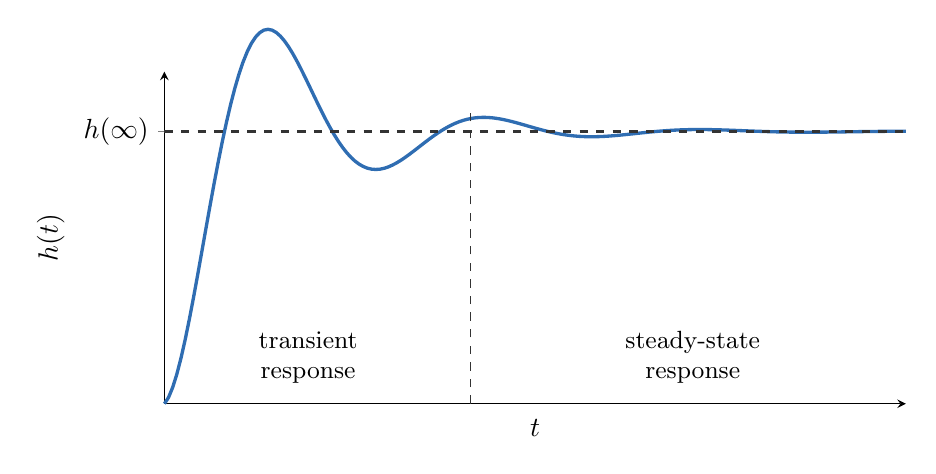
\begin{tikzpicture}
  \begin{axis}[
    width=11cm,
    height=5.8cm,
    xmin=0, xmax=8,
    ymin=0, ymax=1.22,
    axis lines=left,
    xlabel={$t$},
    ylabel={$h(t)$},
    xtick=\empty,
    ytick={1},
    yticklabels={$h(\infty)$},
    every axis plot/.append style={line width=1.2pt, color=lineblue},
    clip=false
  ]
    \addplot[samples=180, domain=0:8] {1 - exp(-0.85*x)*(cos(deg(2.7*x)) + 0.18*sin(deg(2.7*x)))};
    \addplot[dashed, color=linedark] coordinates {(0,1) (8,1)};
    \draw[dashed, color=linedark] (axis cs:3.3,0) -- (axis cs:3.3,1.08);
    \node[font=\small, align=center] at (axis cs:1.55,0.17) {transient\\response};
    \node[font=\small, align=center] at (axis cs:5.7,0.17) {steady-state\\response};
  \end{axis}
\end{tikzpicture}
\end{document}
